\chapter{المجموعة الشمسية}\label{ch:g4:solar-system}

الأرض، كما تعلم، تدور دورة سنوية حول الشمس. لكن أتسافر وحدها؟
ارفع بصرك في مساء صافٍ: بين البريقات الثابتة أضواء ساطعة قليلة
تهيم على مهل من أسبوع إلى أسبوع. سمّاها القدماء الهائمات؛ ونحن
نسمّيها الكواكب --- عوالِمَ تدور حول الشمس نفسها التي ندور
حولها.

\section{نجم واحد وثمانية كواكب}

\begin{definition}[النجم]\label{def:g4:solar-system:star}
\emph{النجم}\index{نجم} كرة هائلة من مادة متوهّجة الحرارة تصنع
ضوءها بنفسها --- أي \omterm{def:g1:light-and-shadows:source}{منبع ضوء} حقيقي. والشمس نجم: نجمنا نحن،
وهي قريبة بما يكفي لتدفئ وجوهنا. (ولنجوم الليل الأخرى فصل خاصّ
بها في السنة القادمة.)
\end{definition}

\begin{definition}[الكوكب]\label{def:g4:solar-system:planet}
\emph{الكوكب}\index{كوكب} عالَم كبير مستدير يسافر حول \omterm{def:g4:solar-system:star}{نجم} ولا
يصنع ضوءًا خاصًّا به --- ونحن نرى الكواكب، كما نرى \omterm{def:g2:moon-in-the-sky:moon}{القمر}، \omterm{def:g1:light-and-shadows:source}{بضوء}
الشمس الذي تردّه. والأرض كوكب.
\end{definition}

\begin{definition}[المجموعة الشمسية]\label{def:g4:solar-system:family}
\emph{المجموعة الشمسية}\index{مجموعة شمسية} هي الشمس مع كل ما
يسافر حولها: الكواكب الثمانية --- وهي بالترتيب: عطارد، والزهرة،
والأرض، والمريخ، والمشتري، وزحل، وأورانوس، ونبتون --- مع
أقمارها وحشد من صخور وكرات جليد أصغر.
\end{definition}

\begin{omfigure}
\begin{tikzpicture}[scale=0.85]
  % the Sun, anchored in the corner
  \fill[omThm] (0,0) -- (0.65,0) arc (0:40:0.65) -- cycle;
  \node[below, font=\small] at (0.45,-0.95) {الشمس};
  % one generous arc of each orbit
  \foreach \r in {1.3, 2.1, 2.9, 3.7, 5.2, 6.9, 8.5, 10.1} {
    \draw[dashed, omExo] (\r,0) arc (0:40:\r);
  }
  % the planets, labels staggered in two rows
  \foreach \r/\name in {1.3/عطارد, 2.9/الأرض, 5.2/المشتري,
      8.5/أورانوس} {
    \fill[omDef] (\r,0) circle (0.11);
    \node[below, font=\footnotesize] at (\r,-0.18) {\name};
  }
  \foreach \r/\name in {2.1/الزهرة, 3.7/المريخ, 6.9/زحل,
      10.1/نبتون} {
    \fill[omDef] (\r,0) circle (0.11);
    \draw[omExo, very thin] (\r,-0.18) -- (\r,-0.72);
    \node[below, font=\footnotesize] at (\r,-0.75) {\name};
  }
\end{tikzpicture}

{\small الشمس وكواكبها الثمانية، بالترتيب --- مرسومة هنا كتفًا
إلى كتف، مع أن كل مدار في الحقيقة أبعد بكثير كثير من الذي
قبله.}
\end{omfigure}

\begin{proposition}[عادات الكواكب]\label{prop:g4:solar-system:habits}
للكواكب عادات مرتّبة: فكل واحد يسافر حول الشمس على طريقه الخاص
الذي يكاد يكون دائريًّا، وكلها تدور في الجهة نفسها، وكل الطرق
تقع في مستوٍ واحد تقريبًا --- مثل حلقات مرسومة على سطح طاولة
واحدة. وكلما بَعُد طريق \omterm{def:g4:solar-system:planet}{الكوكب} عن الشمس طالت دورته الواحدة:
فعطارد يتمّ دورته في $88$ يومًا، والأرض في سنة، ونبتون البعيد
في $165$ سنة.
\end{proposition}

\begin{example}[كواكب صخرية وعمالقة غازية]\label{ex:g4:solar-system:kinds}
الكواكب الأربعة الداخلية --- عطارد والزهرة والأرض والمريخ ---
كرات من صخر، صغيرة صلبة: عوالِم تستطيع أن تقف عليها. والأربعة
الخارجية --- المشتري وزحل وأورانوس ونبتون --- هي
\emph{العمالقة}: كرات هائلة أكثرها \omterm{def:g3:solids-liquids-gases:gas}{غاز} كثيف، ولا أرض فيها تقف
عليها البتة. والمشتري، وهو الأكبر، يستطيع أن يبتلع أكثر من ألف
أرض؛ وزحل يلبس حلقاته اللامعة المشهورة --- وهي قطع جليد صغيرة
لا تُحصى تدور حوله مثل حشد من أقمار دقيقة.
\end{example}

\begin{omfigure}
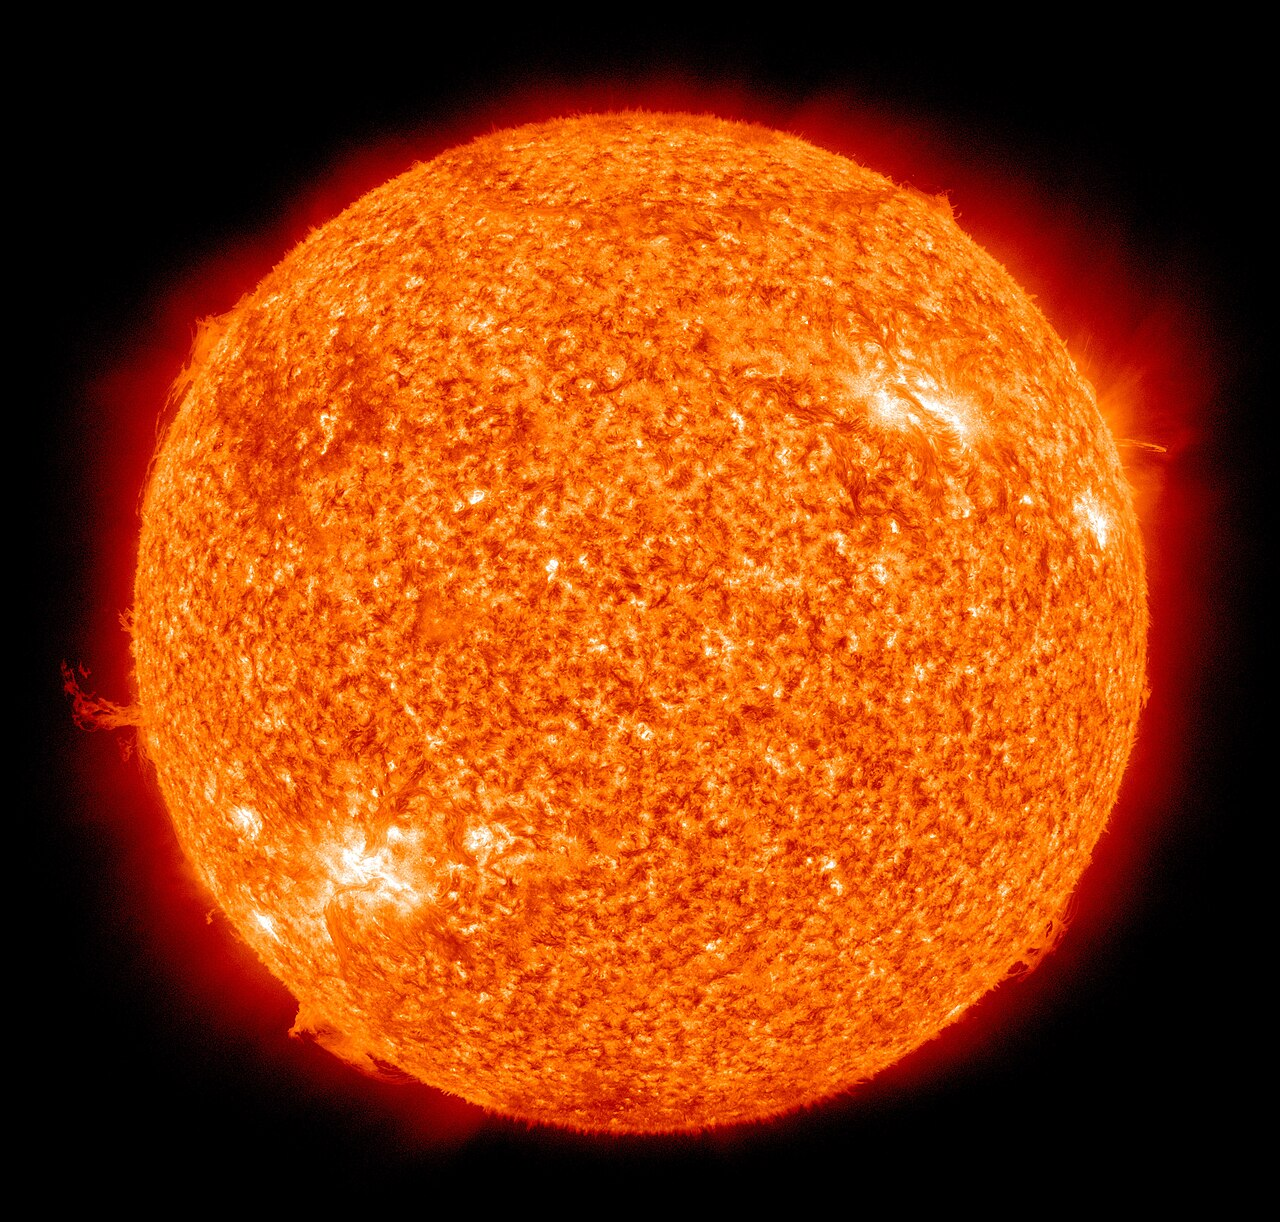
\includegraphics[height=3.1cm]{images/book1/sun-sdo.jpg}

{\small الشمس، نجمنا}

\medskip
\begin{tabular}{cccc}
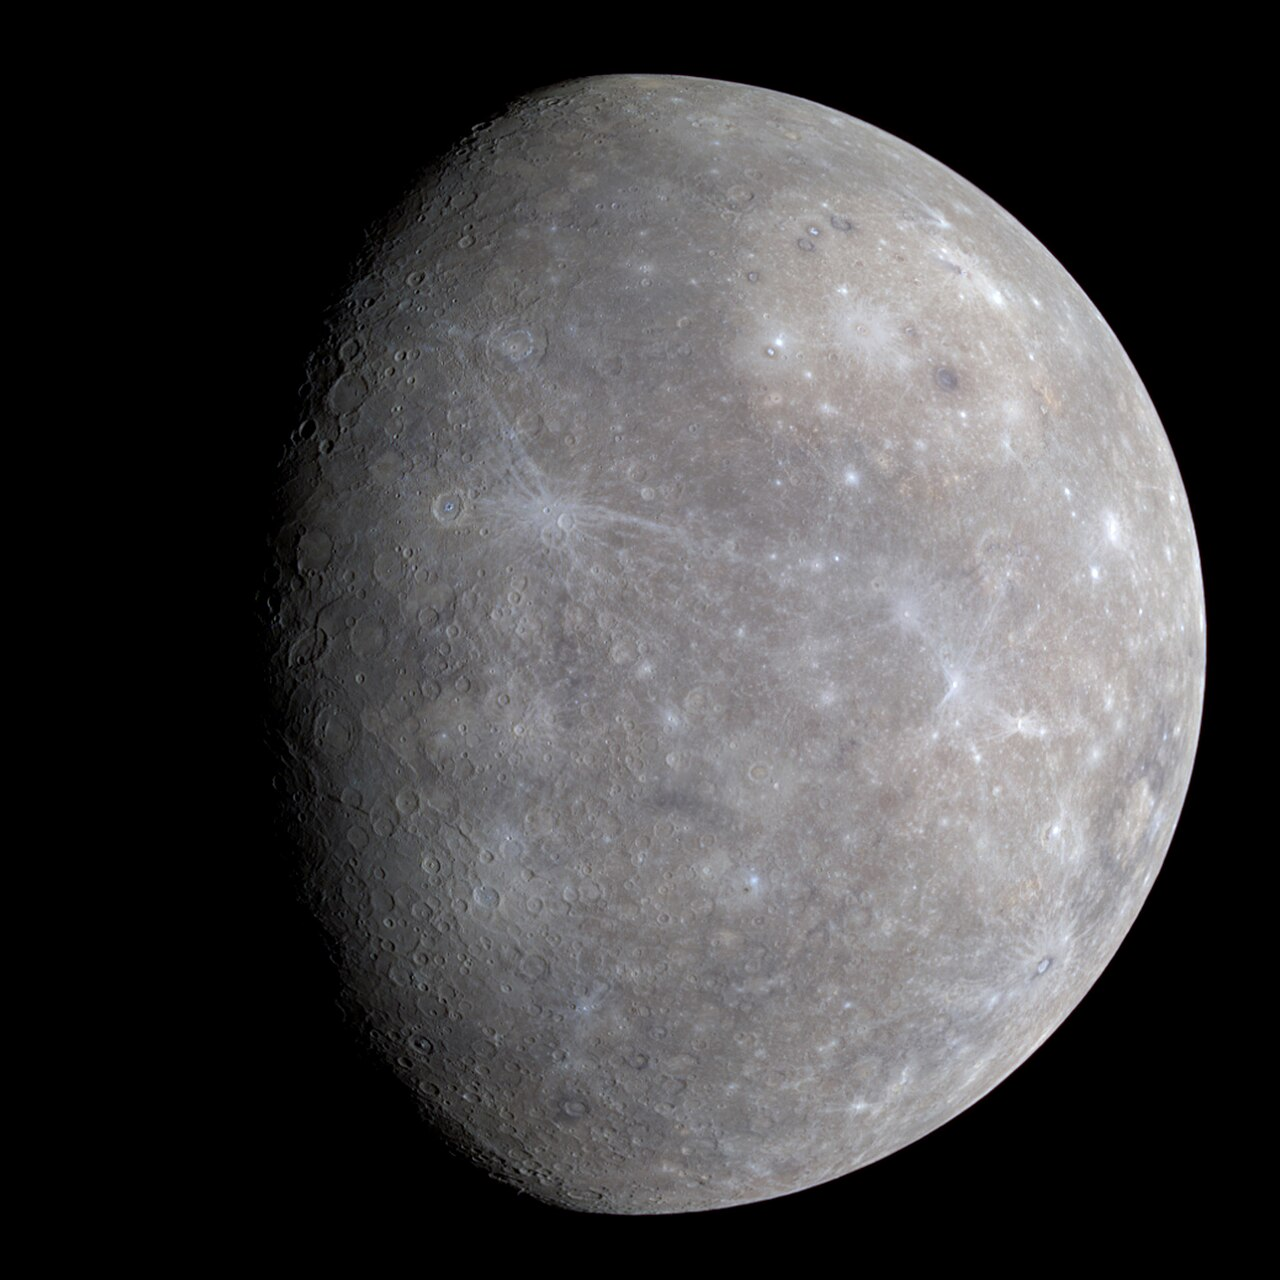
\includegraphics[height=1.75cm]{images/book1/mercury.jpg} &
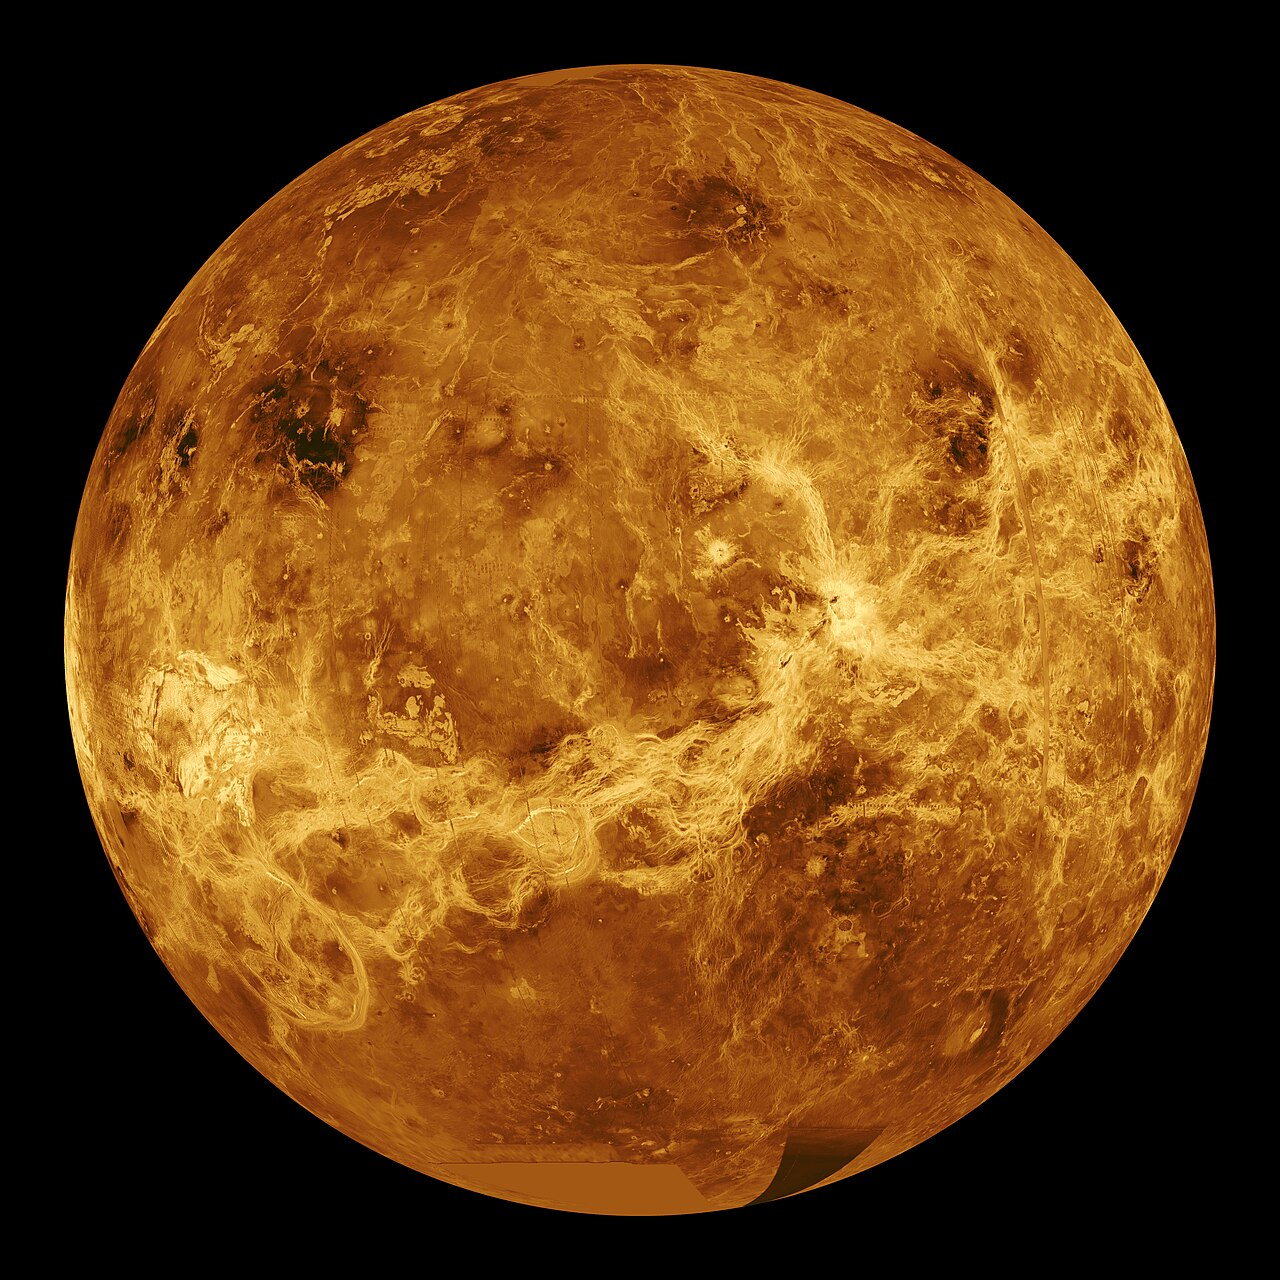
\includegraphics[height=1.75cm]{images/book1/venus.jpg} &
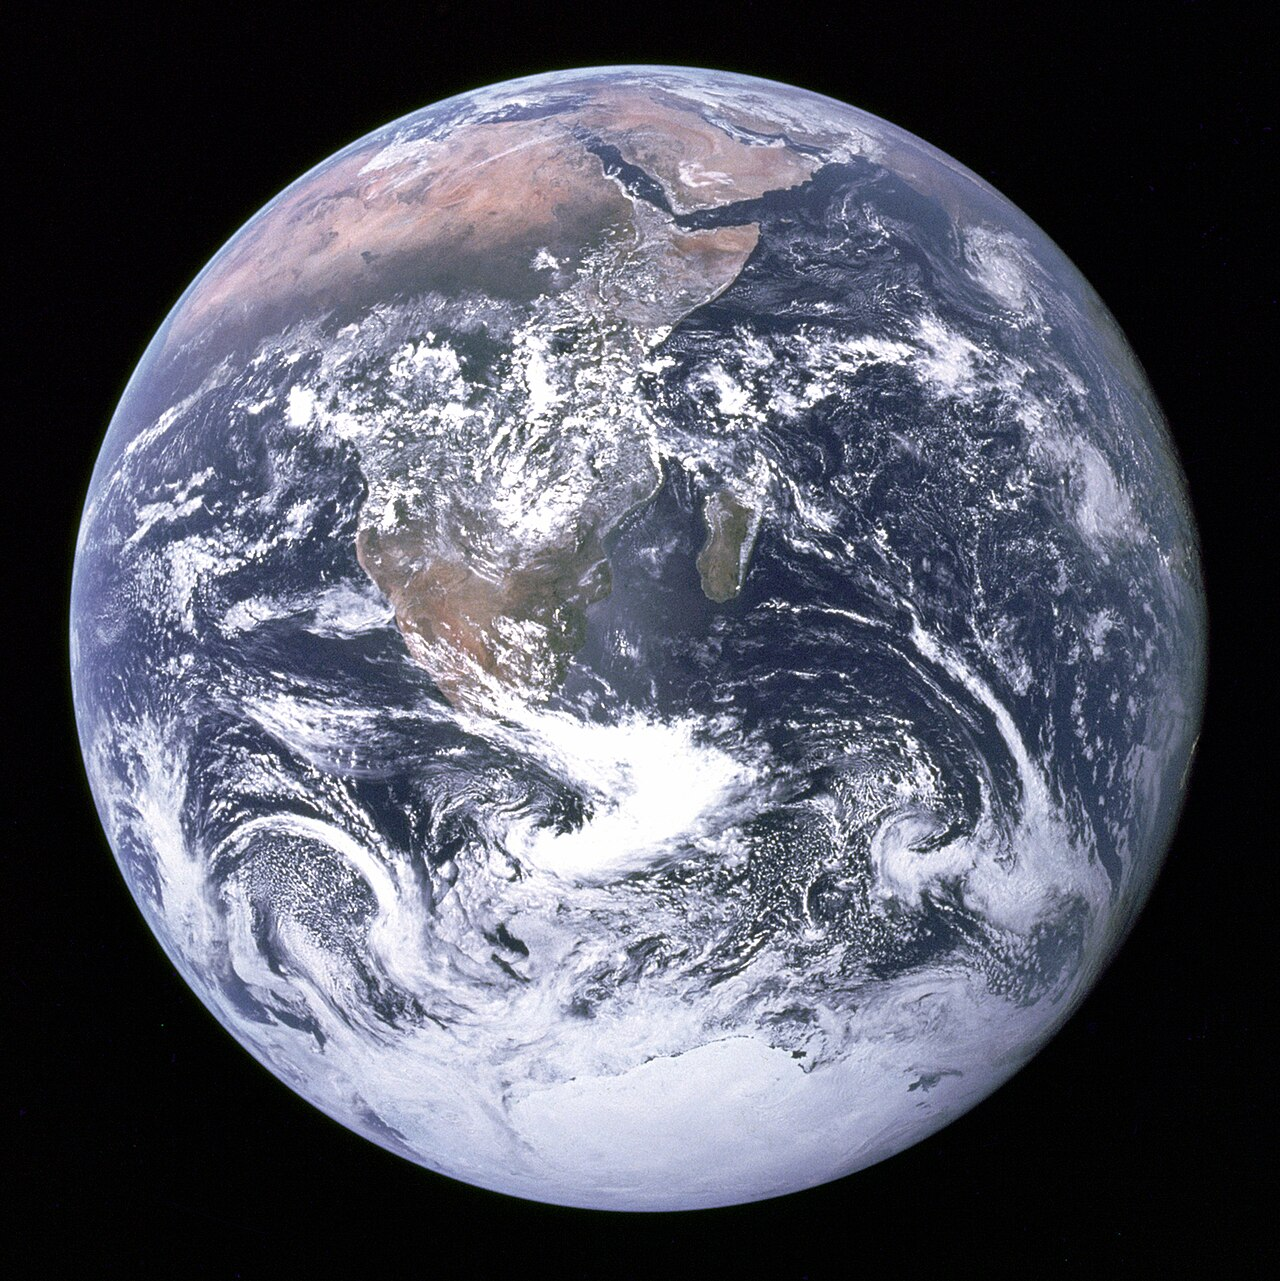
\includegraphics[height=1.75cm]{images/book1/earth.jpg} &
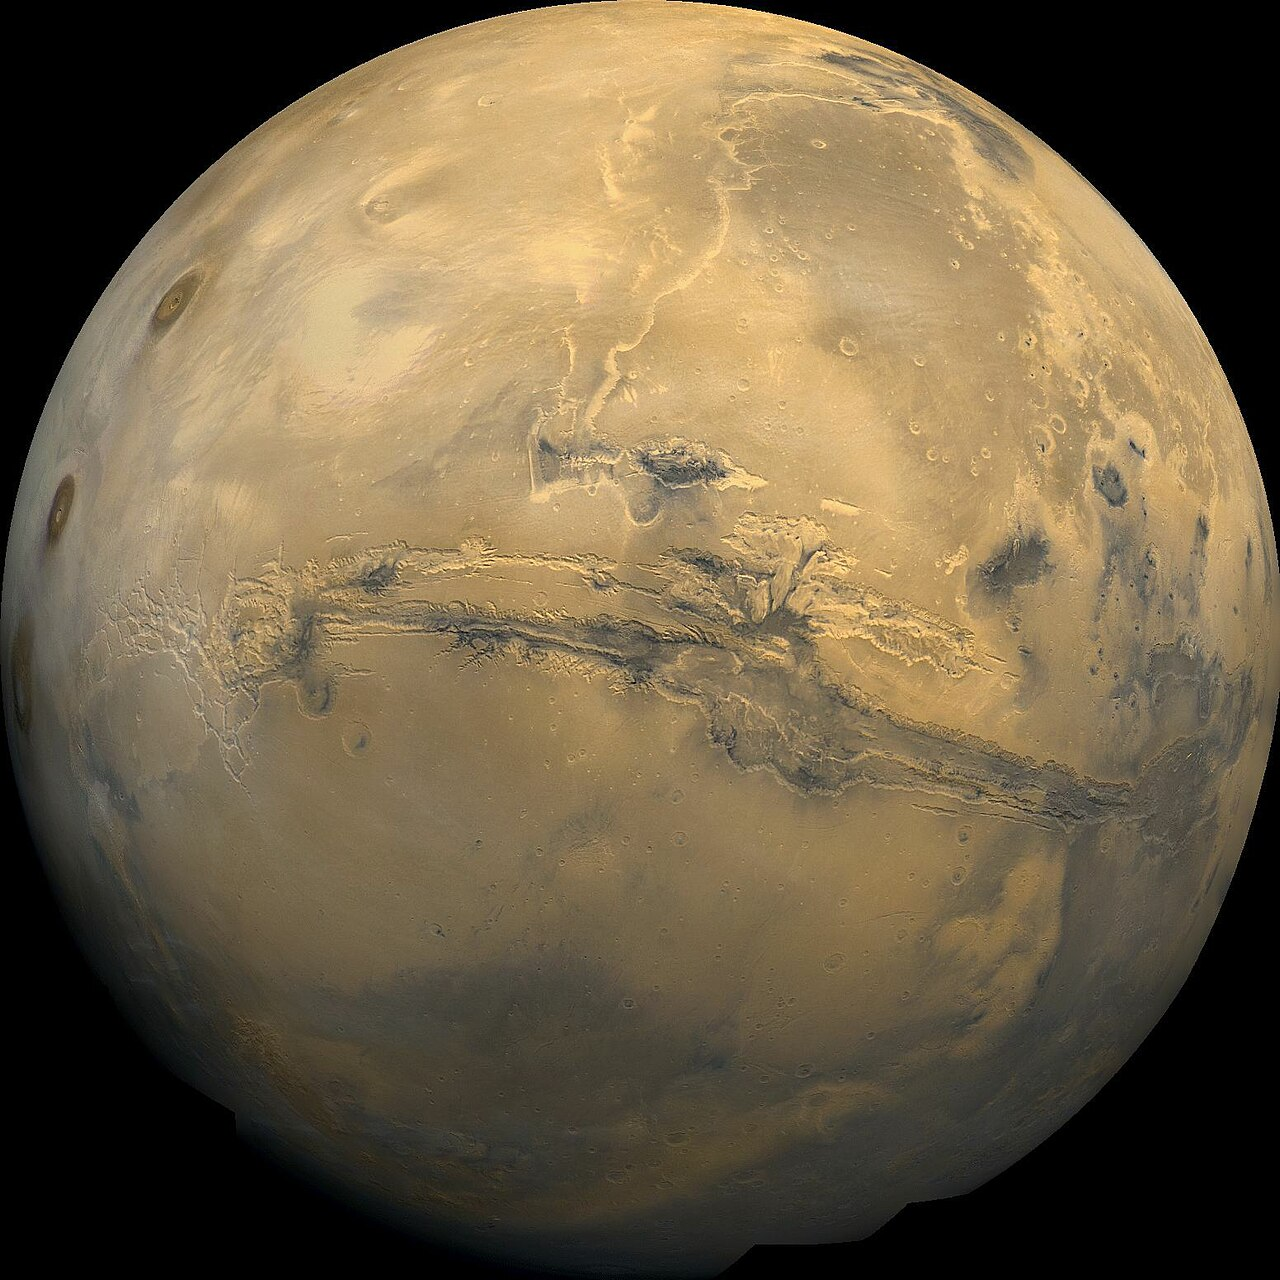
\includegraphics[height=1.75cm]{images/book1/mars.jpg} \\
{\footnotesize عطارد} & {\footnotesize الزهرة} &
{\footnotesize الأرض} & {\footnotesize المريخ} \\[4pt]
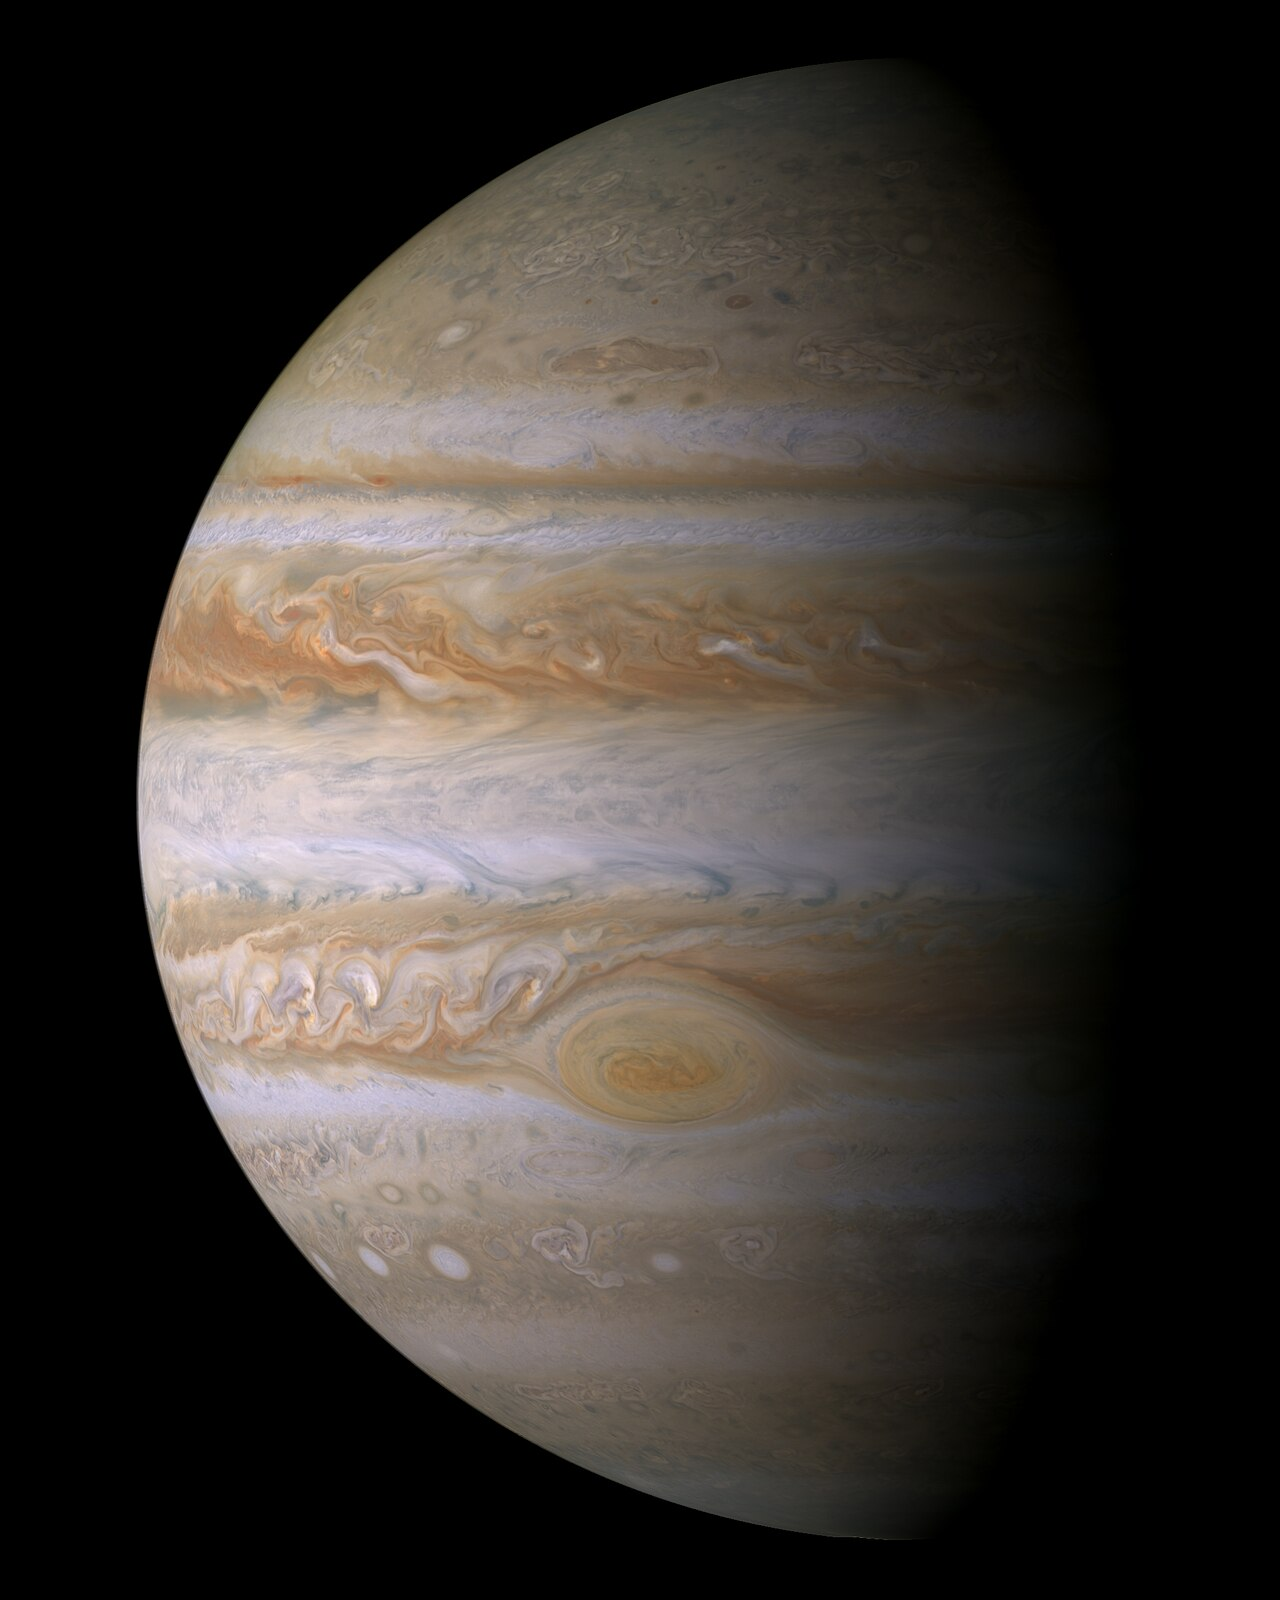
\includegraphics[height=1.75cm]{images/book1/jupiter.jpg} &
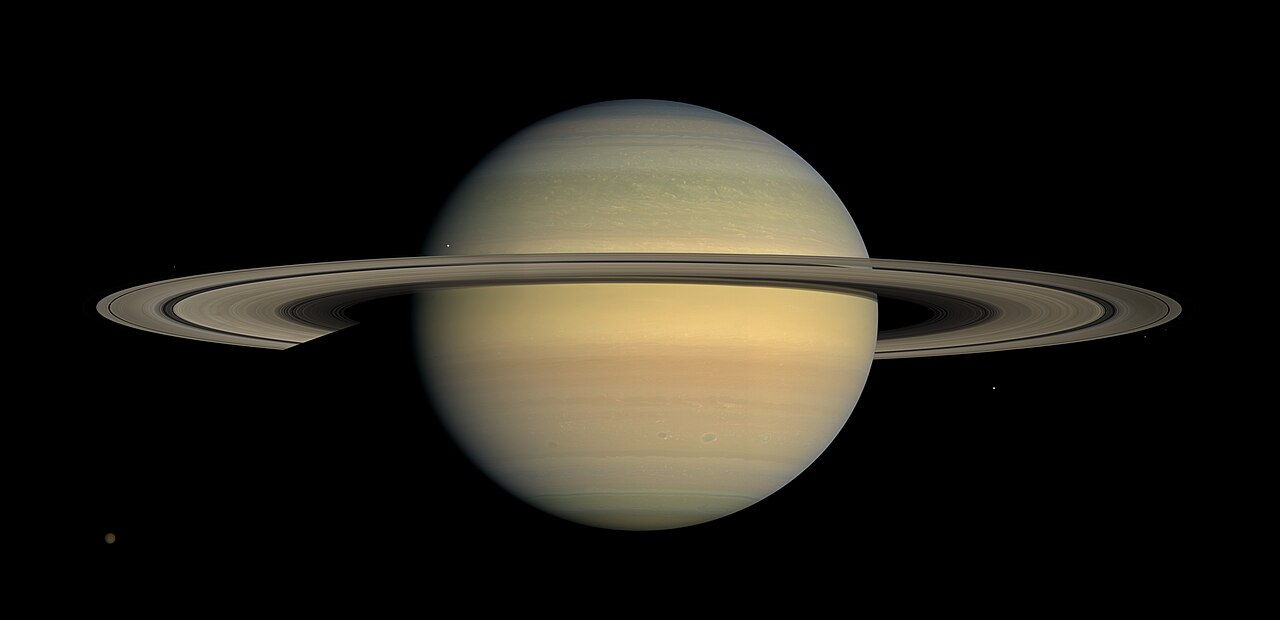
\includegraphics[height=1.75cm]{images/book1/saturn.jpg} &
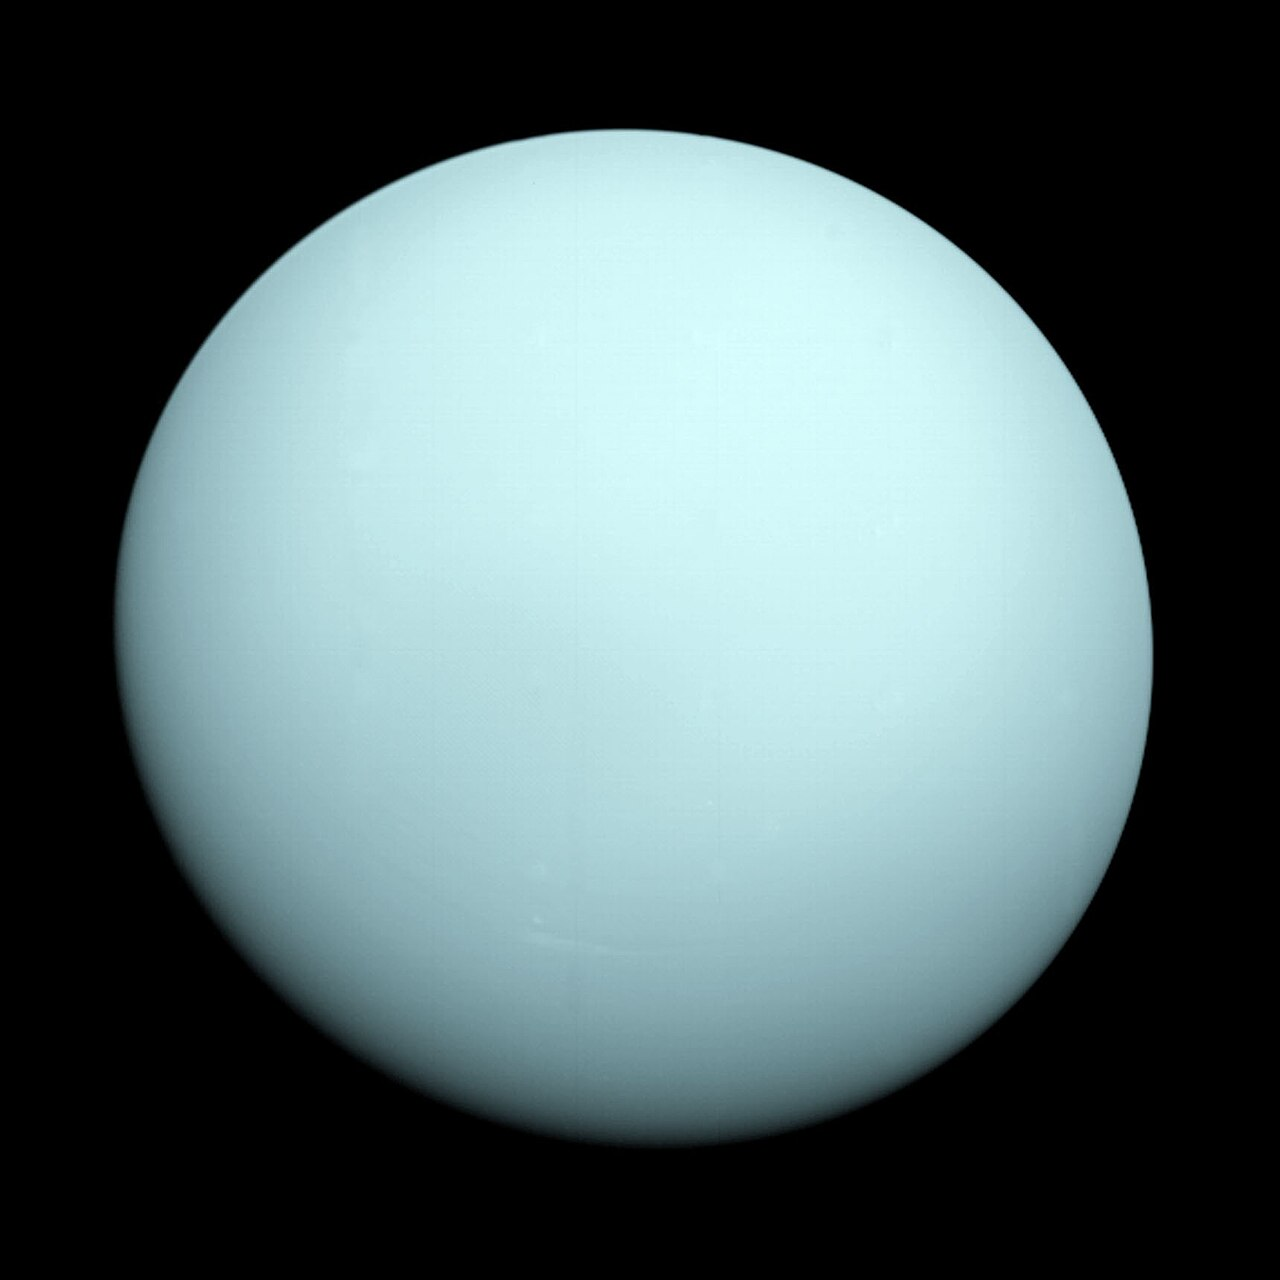
\includegraphics[height=1.75cm]{images/book1/uranus.jpg} &
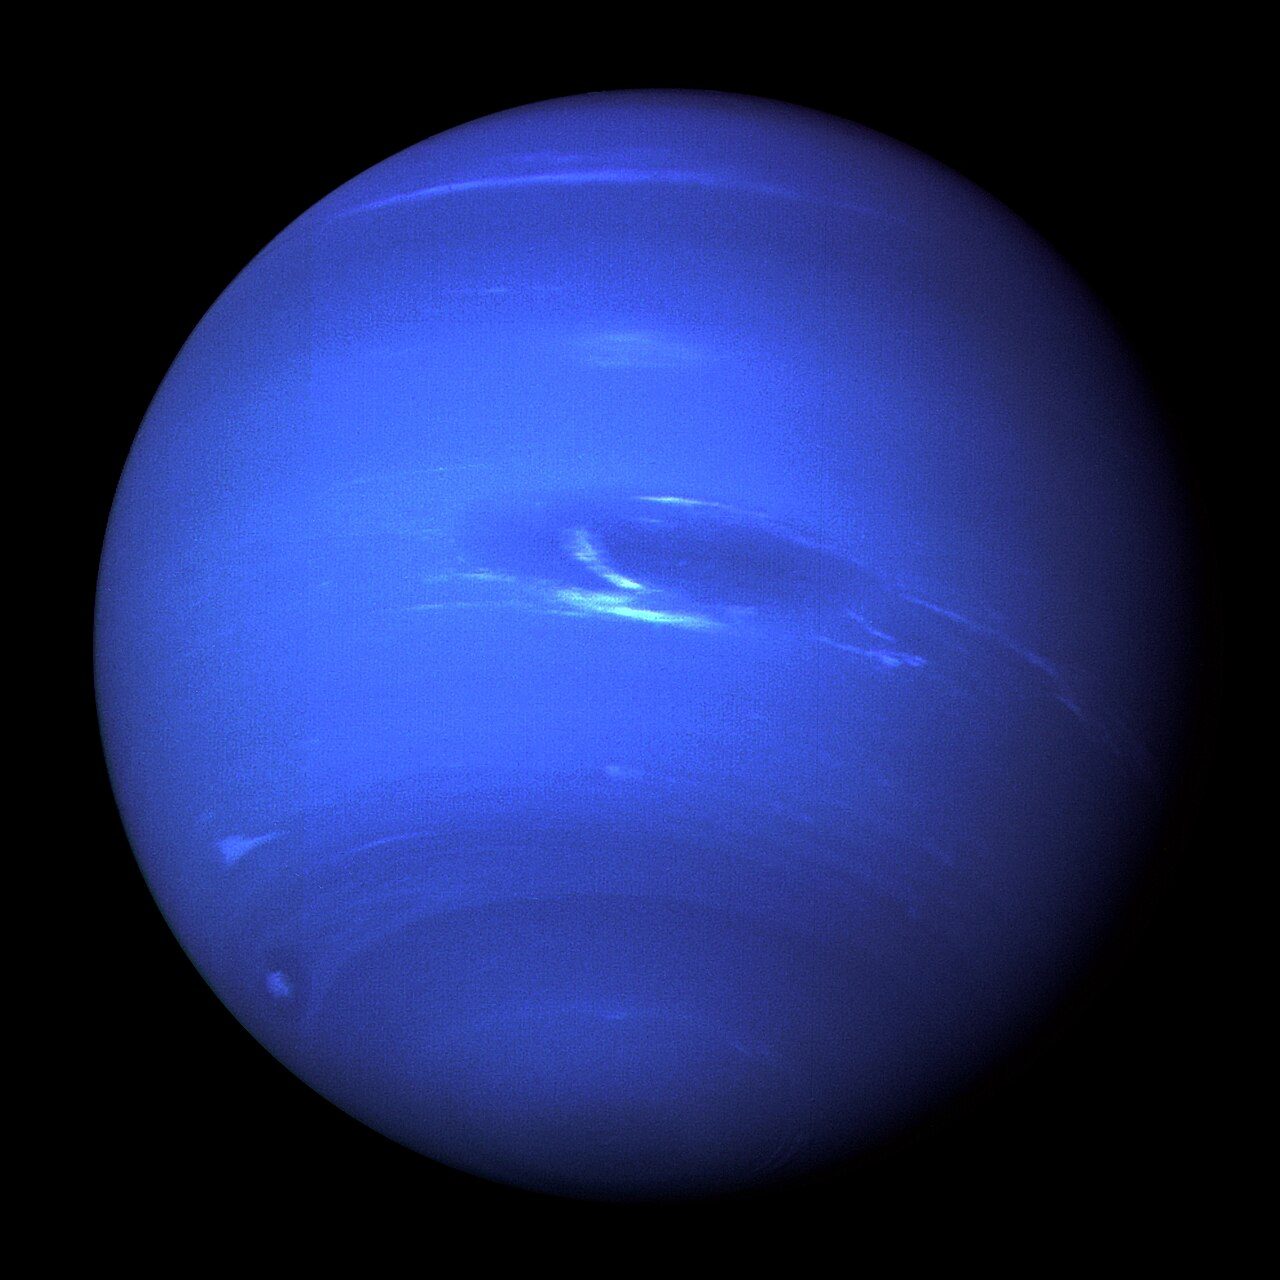
\includegraphics[height=1.75cm]{images/book1/neptune.jpg} \\
{\footnotesize المشتري} & {\footnotesize زحل} &
{\footnotesize أورانوس} & {\footnotesize نبتون}
\end{tabular}

{\small الوجوه الحقيقية للشمس وكواكبها الثمانية، مصوَّرةً
بمسبارات فضائية (والأحجام والمسافات ليست بمقياس واحد؛ والزهرة
معروضة خريطةً بالرادار --- إذ تخفي غيومها الأرض).
\emph{الصور: NASA (ملك عام).}}
\end{omfigure}

\begin{example}[الأقمار ليست كواكب]\label{ex:g4:solar-system:moons}
قمرنا يدور حول \emph{الأرض}، لا حول الشمس مباشرة --- فهو إذن
ليس كوكبًا بل قمرًا، رفيقًا \omterm{def:g4:solar-system:planet}{لكوكب}. ولكواكب أخرى أقمارها الخاصة:
فللمريخ قمران صغيران، وللمشتري وزحل عشرات لكل منهما. \omterm{def:g2:moon-in-the-sky:moon}{فالقمر}
تابع لكوكبه؛ \omterm{def:g4:solar-system:planet}{والكوكب} تابع للشمس.
\end{example}

\section{كم يبلغ البعد}

\begin{method}[نموذج مصغّر للمجموعة الشمسية]\label{met:g4:solar-system:model}
المسافات بين الكواكب هائلة --- ملايين الكيلومترات. ولكي تحسّ
بها، ابنِ نموذجًا مصغّرًا \omterm{def:g4:solar-system:family}{للمجموعة الشمسية} في حديقة، مصغّرًا كل
حجم وكل مسافة بالعامل نفسه:
\begin{enumerate}
  \item اجعل الشمس كرة قدم موضوعة عند البوّابة؛
  \item فتكون الأرض حبّة فلفل --- ولوضعها بعدل، امشِ نحو $30$
        خطوة كبيرة من كرة القدم؛
  \item ويقف عطارد، وهو رأس دبّوس، على نحو $12$ خطوة من كرة
        القدم؛ والمشتري، وهو كرة زجاجية، على نحو $150$ خطوة؛
        ونبتون، وهو خرزة صغيرة، على نحو $900$ خطوة --- أي أكثر
        من نصف كيلومتر بعيدًا!
\end{enumerate}
امشِ المسافة، وتحسّس ما لا يُظهره أي رسم: أن \omterm{def:g4:solar-system:family}{المجموعة الشمسية}
فضاء خالٍ كلها تقريبًا، وفيها عوالِم دقيقة متباعدة جدًّا. وفي
هذا النموذج تمثّل خطوة كبيرة واحدة نحو خمسة ملايين كيلومتر من
الفضاء الحقيقي.
\end{method}

\begin{omfigure}
\begin{tikzpicture}[scale=0.85]
  \draw[-Stealth, thick] (0,0) -- (11.2,0);
  \fill[omThm] (0.5,0) circle (0.3);
  \node[below, font=\footnotesize] at (0.5,-0.42) {كرة قدم};
  \fill[omDef] (1.6,0) circle (0.05);
  \draw[omExo, very thin] (1.6,-0.18) -- (1.6,-0.85);
  \node[below, font=\footnotesize] at (1.6,-0.88) {رأس دبّوس};
  \fill[omDef] (3.2,0) circle (0.08);
  \node[below, font=\footnotesize] at (3.2,-0.35) {حبّة فلفل (الأرض)};
  \fill[omDef] (6.0,0) circle (0.16);
  \draw[omExo, very thin] (6.0,-0.24) -- (6.0,-0.85);
  \node[below, font=\footnotesize] at (6.0,-0.88) {كرة زجاجية (المشتري)};
  \fill[omDef] (10.6,0) circle (0.1);
  \node[below, font=\footnotesize] at (10.6,-0.38) {خرزة (نبتون)};
  \node[above, font=\small] at (5.6,0.5)
    {$12$ خطوة، ثم $30$، ثم $150$، ثم $900$\dots};
\end{tikzpicture}

{\small النموذج المصغّر: صغّر الشمس حتى تصير كرة قدم، فتسع
\omterm{def:g4:solar-system:family}{المجموعة الشمسية} كلها في حديقة --- بالكاد.}
\end{omfigure}

\begin{example}[الهائمات في سمائنا]\label{ex:g4:solar-system:wanderers}
الزهرة كثيرًا ما تكون أول ``\omterm{def:g4:solar-system:star}{نجم}'' في المساء، متوهّجة في الغرب
بعد \omterm{def:g1:day-and-night:daynight}{الغروب} --- وهي بهذا السطوع لأنها أقرب جيراننا، ملفوفة
بغيوم بيضاء تردّ \omterm{def:g1:light-and-shadows:source}{ضوء} الشمس ردًّا سخيًّا. والمريخ يتوهّج
برتقاليًّا خافتًا؛ والمشتري وزحل يسطعان سطوعًا ثابتًا ساطعًا.
راقب واحدًا منها بضعة أسابيع في مواجهة النجوم الثابتة: تجده
ينزاح --- وهو الهيام بعينه الذي أعطى الكواكب اسمها القديم.
\end{example}

\begin{remark}[صورة قديمة أُعيد رسمها]\label{rem:g4:solar-system:history}
كان الناس في معظم التاريخ يضعون الأرض في مركز كل شيء، والشمس
\omterm{def:g2:moon-in-the-sky:moon}{والقمر} والكواكب تدور حولنا. لكن المتأنّين في مراقبة الهائمات
وجدوا تلك الصورة تئنّ --- فالكواكب تنزاح أحيانًا \emph{إلى
الوراء} \omterm{def:g2:measuring-time:duration}{مدة}، ويصعب تفسير ذلك والأرض متوّجة في الوسط. أما الصورة
التي تتوسّطها الشمس، وقد تعلّمتها توًّا، ففسّرت الهيام تفسيرًا
بسيطًا، وهي من أجرأ الأفكار التي قبلها البشر يومًا: أن بيتنا
ليس المركز --- إنما هو \omterm{def:g4:solar-system:planet}{الكوكب} الثالث من الشمس.
\end{remark}

\section{تمارين}

\begin{exercise}[$\star$]\label{exo:g4:solar-system:1}
ما الفرق بين \omterm{def:g4:solar-system:star}{النجم} \omterm{def:g4:solar-system:planet}{والكوكب}؟ وأيّهما الشمس؟ وأيّهما الأرض؟
\end{exercise}

\begin{exercise}[$\star$]\label{exo:g4:solar-system:2}
اذكر الكواكب الثمانية بالترتيب من الشمس. وأيّها كوكبنا؟
\end{exercise}

\begin{exercise}[$\star$]\label{exo:g4:solar-system:3}
أيّ الكواكب صغيرة صخرية؟ وأيّها العمالقة الغازية؟ وسمِّ أكبرها
جميعًا، والذي له الحلقات المشهورة.
\end{exercise}

\begin{exercise}[$\star$]\label{exo:g4:solar-system:4}
لماذا لا يُعدّ \omterm{def:g2:moon-in-the-sky:moon}{القمر} من الكواكب؟ وحول أيّ شيء يدور؟
\end{exercise}

\begin{exercise}[$\star$]\label{exo:g4:solar-system:5}
يتمّ عطارد دورته حول الشمس في $88$ يومًا، والأرض في $365$،
ونبتون في $165$ سنة. فأيّ عادة من عادات الكواكب تبيّنها هذه
الأعداد؟
\end{exercise}

\begin{exercise}[$\star$]\label{exo:g4:solar-system:6}
في النموذج المصغّر في الحديقة، ما الذي يمثّل الشمس، وعلى كم
خطوة تقف الأرض؟ ومِمّ تتألّف \omterm{def:g4:solar-system:family}{المجموعة الشمسية} كلها تقريبًا من
حيث الحيّز؟
\end{exercise}

\begin{exercise}[$\star$]\label{exo:g4:solar-system:7}
الزهرة تسطع سطوعًا باهرًا، ومع ذلك ليست نجمًا. فمن أين يأتي
ضوءها؟ (يجيب صديق قديم: فكّر في \omterm{def:g2:moon-in-the-sky:moon}{القمر}.)
\end{exercise}

\begin{exercise}[$\star$]\label{exo:g4:solar-system:8}
كيف تعرف، بمراقبة السماء بضعة أسابيع، أن ضوءًا ساطعًا \omterm{def:g4:solar-system:planet}{كوكب} لا
\omterm{def:g4:solar-system:star}{نجم}؟
\end{exercise}

\begin{exercise}[$\star$]\label{exo:g4:solar-system:9}
في نموذج الحديقة يقف المشتري على نحو $150$ خطوة والأرض على نحو
$30$. فكم مرة تقريبًا يكون المشتري أبعد عن الشمس من الأرض؟
\end{exercise}

\begin{exercise}[$\star\star$]\label{exo:g4:solar-system:10}
يرسم صديق \omterm{def:g4:solar-system:family}{المجموعة الشمسية} والكواكب الثمانية كلها محشورة حول
الشمس مثل صورة الفصل الأولى، ويسأل لماذا تستغرق المسبارات سنوات
لتبلغ الكواكب الخارجية. صحّح له الأمر بالنموذج المصغّر في
الحديقة --- في أيّ شيء تكذب كل رسوم \omterm{def:g4:solar-system:family}{المجموعة الشمسية} تقريبًا،
ولماذا تضطرّ إلى ذلك؟
\end{exercise}

\begin{exercise}[$\star\star$]\label{exo:g4:solar-system:11}
حين كان يُعتقد أن الأرض في مركز كل شيء، أيّ أحجية من أحاجي
مراقبة السماء كانت تئنّ في وجه تلك الصورة؟ وكيف حلّ وضعُ الشمس
في المركز الأحجيةَ --- وماذا كلّفتنا الصورة الجديدة من كبرياء؟
\end{exercise}
